%!TEX root = ../thesis.tex
% This paragraph covered a lot of ground, but I was a bit lost since each sentence tried to cover too many different approaches. Is there an implied structure? E.g. first software-static, then software-video, then physical tasks? Id’ have expected some more basic references early on that for example show that people don’t read software documentation and instead look for task-centered learning materials. There’s also a difference between related work that investigates what good instruction formats are, and systems work that introduces new tools to create such formats.

\chapter{Background}
\label{chapter_background}

This dissertation proposes computational methods to create interactive tutorials for software applications and physical tasks. To ground our work in existing practices and principles, in this chapter, I define the terminology commonly used by tutorial researchers and online community (Section \ref{background_terms}).
%
I survey research studies and literature about the motivations of people creating, sharing, and consuming tutorials (Section \ref{background_why}) and a common creation process (Section \ref{background_creation}).

% -------------------------------------------

\section{Instructions: Terminology}
\label{background_terms}

A \keyword{tutorial}, or a \keyword{how-to}, is a representation that transfers domain-specific \keyword{know-how} by describing a set of \keyword{instructions} on how to accomplish a specific \keyword{task}. Instructions have been widely created for various domains, including:

\begin{itemize}
  \itemsep -2pt
  \item Software applications, such as manipulating an image to create a specific blurring effect or creating a pie chart using a spreadsheet application,
  \item Do-It-Yourself (DIY) projects, such as wrapping a gift box or assembling a piece of furniture,
  \item Everyday activities, such as cooking or operating a vacuum machine, and
  \item Sports, such as making a dance move or swing a golf club.
\end{itemize}

Figure~\ref{fig:background_activities} shows example activities of the above domains from online video tutorials.
\\

% A task-centric tutorial often involves domain-specific \keyword{know-how}, knowledge that is required to perform a task.
%
Instructional content is commonly structured as a list of \keyword{steps} or \keyword{subtasks} in a linear, \keyword{step-by-step} order.
%
In some domains, instructions have been derived into specific formats. For example, cooking recipes contain not only actions but also food ingredients and required amounts.
% The term \keyword{recipe} has been used for activities other than cooking.

Note that instructions are different from a (software) \keyword{documentation}, \keyword{manual}, or \keyword{user guide}, which is a technical document contained non-task-centric details about a particular hardware or software system. A manual does not provide step-by-step guidance to follow. To accomplish a task, one needs to identify relevant information from the documentation and reason the workflow.

\begin{figure*}[t]
  \centering
  \begin{minipage}{\textwidth}
  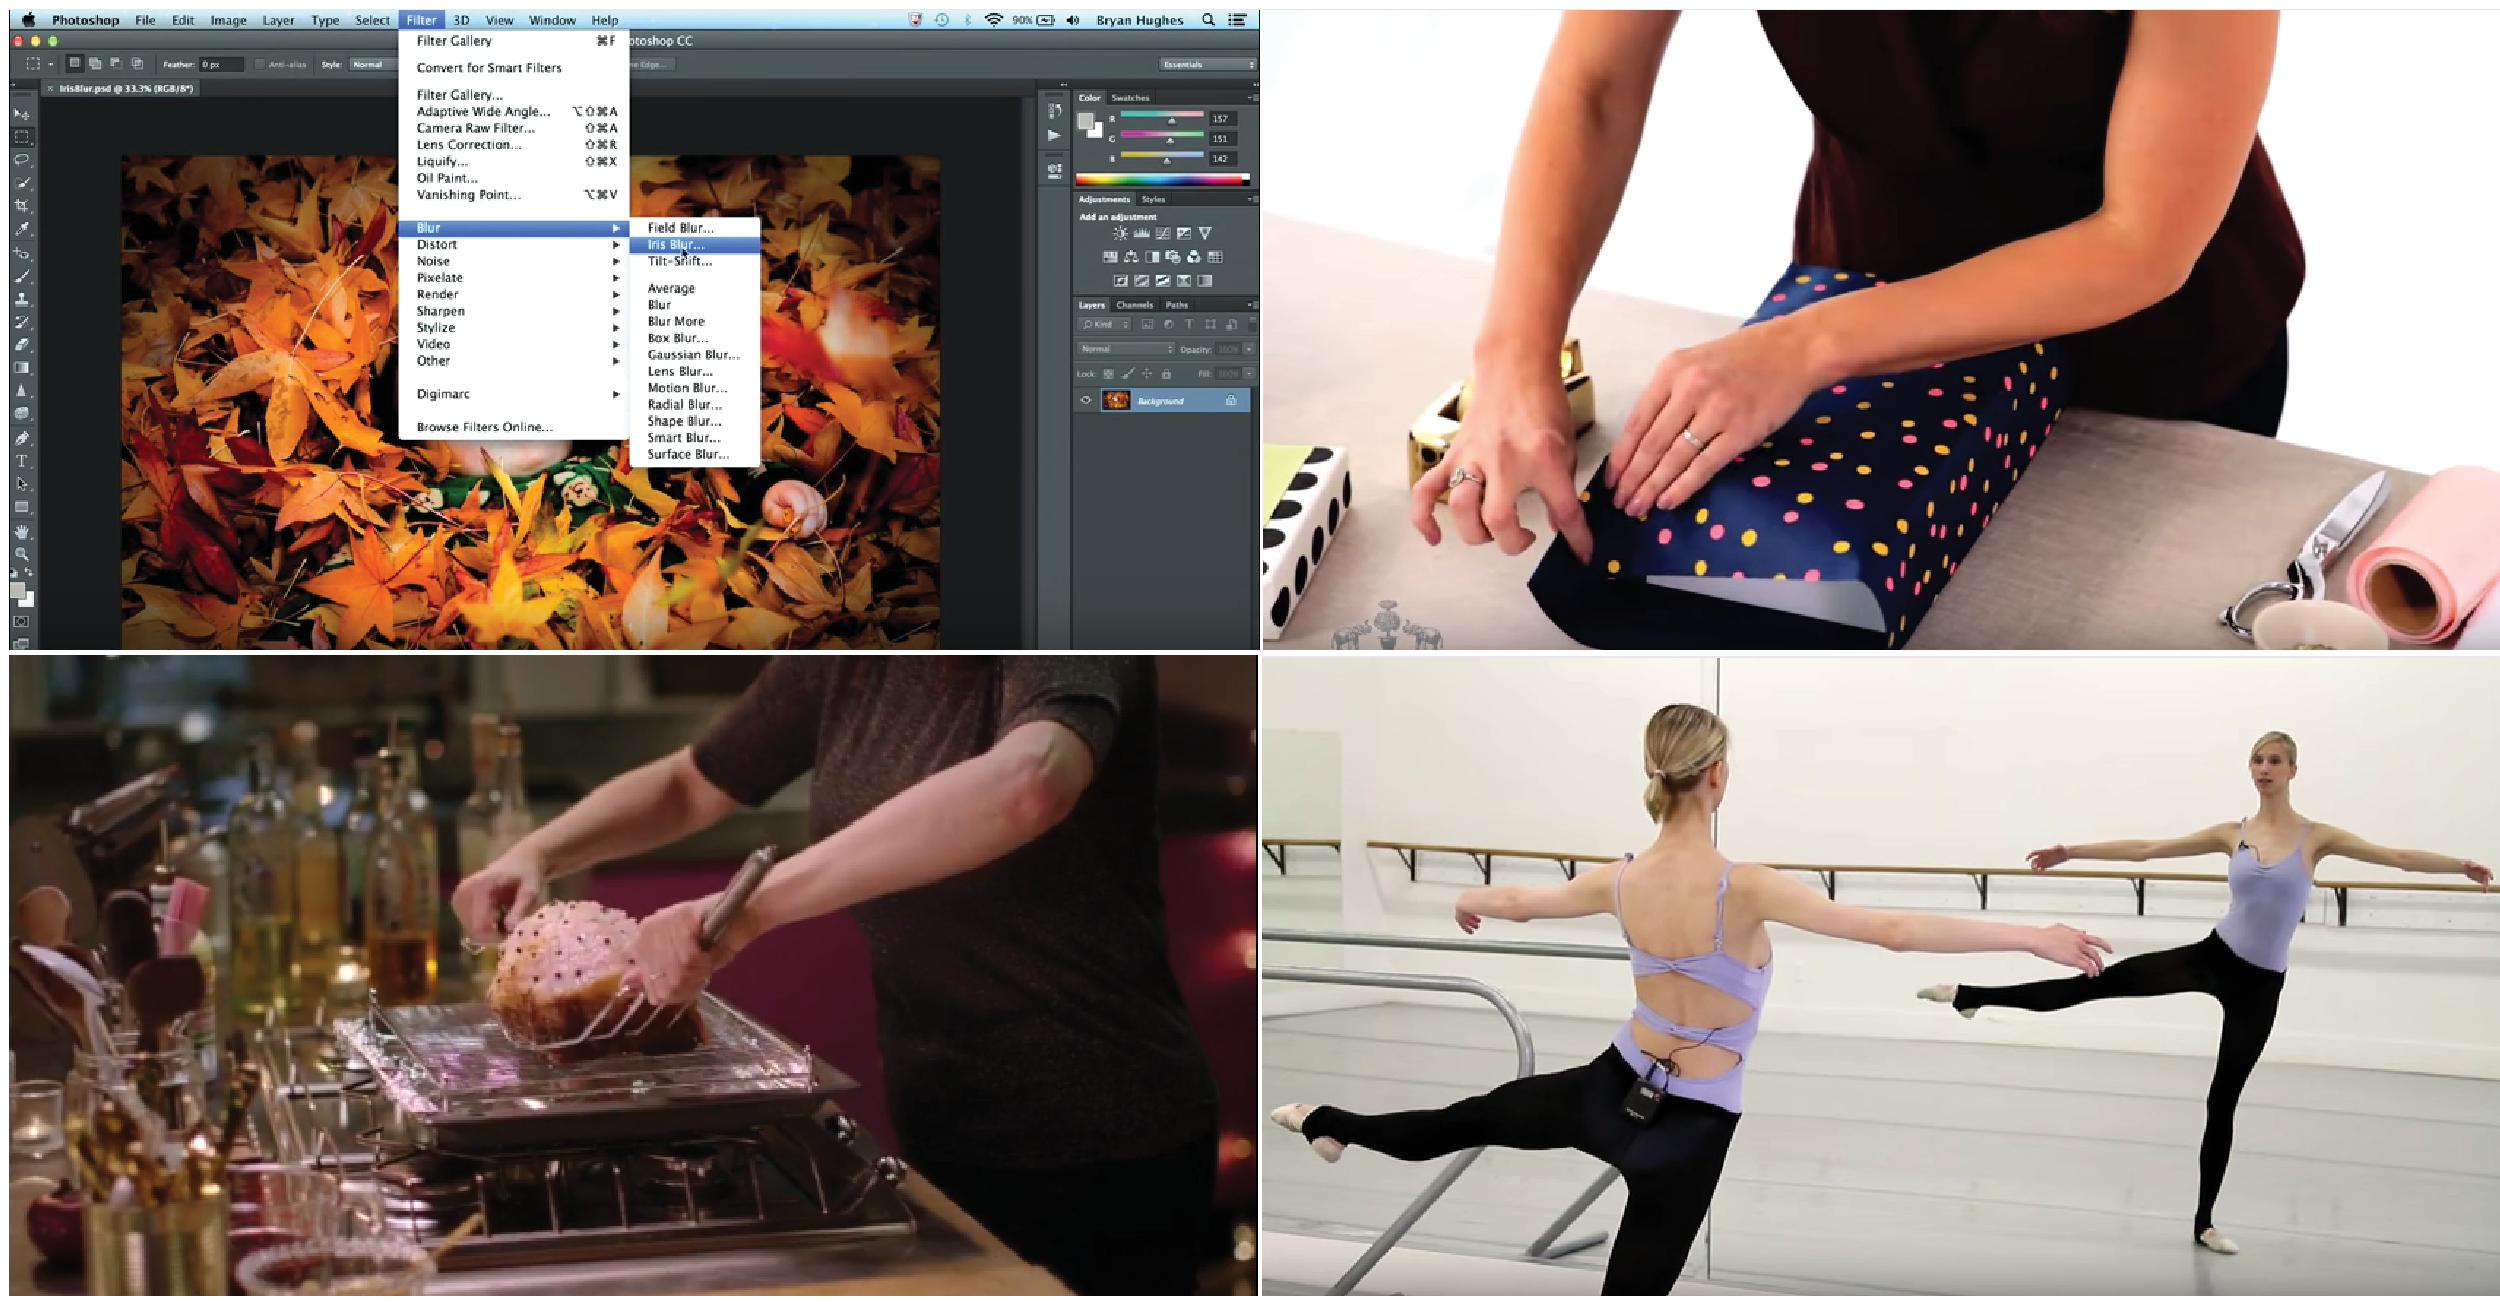
\includegraphics[width=\textwidth]{\background/fig/activities/activities}
  \caption[activities]{Example activities in tutorial domains:
  %
  a) image manipulations using a software application
  \footnote{Photoshop Playbook: Selective Focus \url{https://youtu.be/Wh3ahxqDnyw}},
  %
  b) wrapping a gift, a DIY task
  \footnote{One Kings Lane: How to Wrap the Perfect Gift \url{https://youtu.be/Me3ykrZobJE}},
  %
  c) cooking, an everyday activity
  \footnote{Slow-cooked black treacle ham \url{http://www.bbc.co.uk/food/recipes/slow-cooked_black_21152}}, and
  %
  d) ballet dancing in sports
  \footnote{Ballet 101: How to Do the Fouette in Ballet Dancing \url{https://youtu.be/DzqQNlaahjs}}.
  }
  \label{fig:background_activities}
  \end{minipage}
\end{figure*}

% -------------------

Instructions can be shown in different forms. There are two main forms of visual tutorials (see Figure~\ref{fig:background_format}):
\begin{itemize}
  \itemsep -2pt
  \item \keyword{Static tutorials}, which use text and figures to describe the set of operations required to accomplish a task. Such format is presented as a written document with a step-by-step list, while each step includes text description and/or an image or abstract \keyword{illustration} to describe the subtask. It can possible be combined into a \keyword{diagram} that shows the flow in a pictorial form. Static tutorials are suitable for printing and are easy to scan because they show all instructions.
  \item \keyword{Video tutorials}, which are edited or raw videos of the tutorial author performing the the task. Examples include screen recordings of a software application or a camera recording of a DIY task.
\end{itemize}

\begin{figure*}[t]
  \centering
  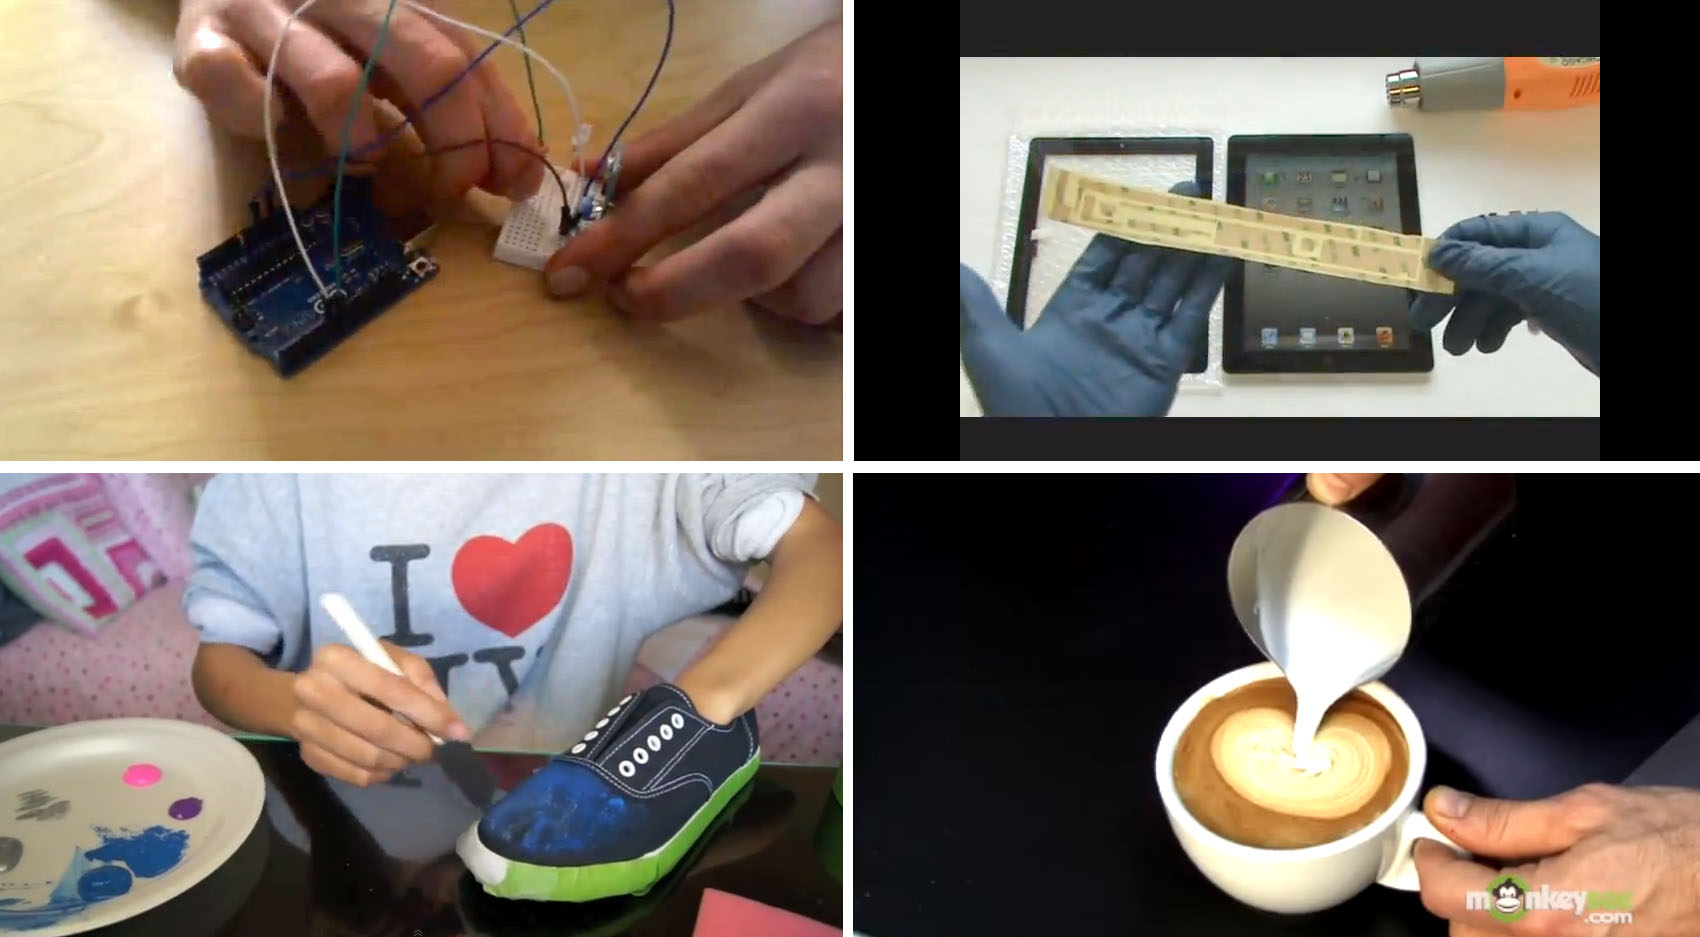
\includegraphics[width=\textwidth]{\background/fig/tutorials}
  \caption{Tutorial formats. \tofix{update the fig}}
  \label{fig:background_format}
\end{figure*}

% -------------------

\subsection{Creating Instructions}
Instructions are created by one or more \keyword{authors} who document the process of completing a task and refine the material to a final deliverable.
%
Since the process often involves innovations and creations, authors can also be referred as \keyword{creators}, \keyword{makers}, or \keyword{hobbyists}.
%
Instructional authors are often the \keyword{professionals} or \keyword{experts} in the domains of their work. However, in tutorial production, they might be \keyword{amateurs} or \keyword{novices} who are not familiar with software tools to refine the documented material.

Throughout this dissertation, we call the process of author completing a task as a \keyword{demonstration} or a \keyword{performance}. Authors can therefore be as \keyword{demonstrators} or \keyword{presenters}.
%
In software, the demonstration process can be referred as a system \keyword{walkthrough}. Section \ref{background_creation} will discuss the \keyword{production} process of instructions.

% -------------------

\subsection{Consuming Instructions}
We define people who review instructional content as \keyword{viewers} or \keyword{learners}. Viewers may also be \keyword{followers} if they choose to follow the instructions to achieve the same or similar tasks.
%
Studies have shown that learners with different learning needs and habits have various preference on the tutorial formats. In Chapter \ref{chapter_mixt}, I'll examine these differences and propose a new instructional format.

% lecturer and online tutoring: involve more feedback collection and response to learners, beyond the scope of this paper

% -------------------------------------------

\section{Why Instructions?}
\label{background_why}

The research community has been investigating the motivations of both authors and viewers of how-to videos and written tutorials. While one primary motivation is to share expertise, published videos also serve as a way to broadcast skill and as an online portfolio~\cite{Torrey:2007he,Kuznetsov:2010:REA:1868914.1868950}. Authors may derive revenue through advertising or referrals~\cite{Lafreniere:2012tl}. Viewers, on the other hand, typically seek technical explanations, but are also searching for inspiration~\cite{Torrey:2009fc} and looking for validation of existing skills~\cite{Lafreniere:2012tl}.
%
These studies suggest that tutorials have a larger variety of purposes and uses than merely communicating technical content. Recently, guidelines of improving tutorial authorship have been proposed \cite{Wakkary:2015:TAH:2702123.2702550}. Key findings include identifying tools and components and structuring a task into steps with a clear sequence. In our work, we strive to make authoring of instructions more accessible to amateurs while maintaining opportunities for adding individual style through control over editing effects.

Instructables: \cite{Tseng:2014:PVP:2598510.2598540}

% people don’t read software documentation and instead look for task-centered learning materials

% -------------------------------------------

\section{Instruction Production Process}
\label{background_creation}

Creating instructions can involve several stages, especially for activities that require more steps and time \tofix{studies here}.
%
Figure~\ref{fig:background_creation} shows a common workflow of tutorial creation:

\begin{itemize}
  \item \parTitleBold{Planning}:
    Authors make a
  \item \parTitleBold{Capturing}:
    Mutlimedia material is often used to document a process:
    \begin{itemize}
      \itemsep -2pt
      \item Static photographs capture specific moments in a procedure.
      \item Video footages record a computer screencast or a scene of a demonstration.
      \item Audio recordings preserve the sound of activities or author narration.
      \item Other domain-specific content (e.g., code, board layouts, 3D models, and sketches) or resources (e.g., books or URLs to other material) often enrich the instructions.
    \end{itemize}
  \item \parTitleBold{Editing}:
    Once ... to make it in a readable or viewable form
  \item \parTitleBold{Reviewing}:
  \item \parTitleBold{Releasing/Sharing}:
    Finally, authors may release the refined content and share the deliverable with others. Common media or platforms include: personal blogs, content sharing sites (e.g., YouTube, Instructables), forums, emails, or private networks.
\end{itemize}

Some tutorial creators, especially professionals, may work as a team with multiple role players in a production process, while some work individually. The time required to create a tutorial may vary from a few minutes to weeks.
% , depending on the stages involved and the content.

\begin{figure*}[t]
  \centering
  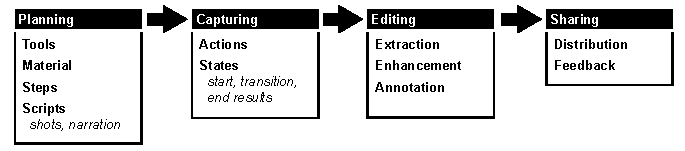
\includegraphics[width=\textwidth]{\background/fig/creation_process}
  \caption{A common workflow of tutorial creation. \tofix{update the fig}}
  \label{fig:background_creation}
\end{figure*}
